\documentclass[a4paper]{article}
\usepackage[spanish]{babel}
\usepackage[utf8]{inputenc}
\usepackage[T1]{fontenc}
\usepackage{charter}  % tipografia
\usepackage{graphicx}
\usepackage{float}
\usepackage{amsmath, amsthm, amssymb}
%\usepackage{inconsolata}
\usepackage{clrscode}
\usepackage{underscore}
\usepackage{caratula}
\usepackage{listings}
\usepackage{array}
\usepackage{color} % para snipets de codigo coloreados
\usepackage{fancybox} % para el sbox de los snipets de codigo
\definecolor{litegrey}{gray}{0.94}
% \newenvironment{sidebar}{%
% \begin{Sbox}\begin{minipage}{.85\textwidth}}%
% {\end{minipage}\end{Sbox}%
% \begin{center}\setlength{\fboxsep}{6pt}%
% \shadowbox{\TheSbox}\end{center}}
% \newenvironment{warning}{%
% \begin{Sbox}\begin{minipage}{.85\textwidth}\sffamily\lite\small\RaggedRight}%
% {\end{minipage}\end{Sbox}%
% \begin{center}\setlength{\fboxsep}{6pt}%
% \colorbox{litegrey}{\TheSbox}\end{center}}

%\newenvironment{codesnippet}{%
%\begin{Sbox}\begin{minipage}{\linewidth-2\fboxsep-2\fboxrule-4pt}\sffamily\small}%
%{\end{minipage}\end{Sbox}%
%\begin{center}%
%\colorbox{litegrey}{\TheSbox}\end{center}}

% \newenvironment{codesnippet}{\VerbatimEnvironment%
%   \noindent
%   %{\columnwidth-\leftmargin-\rightmargin-2\fboxsep-2\fboxrule-4pt}
%   \begin{Sbox}
%   \begin{minipage}{\linewidth-2\fboxsep-2\fboxrule-4pt}
%   \begin{Verbatim}
% }{%
%   \end{Verbatim}
%   \end{minipage}
%   \end{Sbox}%
%   \colorbox{litegrey}{\TheSbox}
% }

\newenvironment{codesnippet}{\VerbatimEnvironment%
  \noindent
  %      {\columnwidth-\leftmargin-\rightmargin-2\fboxsep-2\fboxrule-4pt}
  \begin{Sbox}
  \begin{minipage}{\linewidth}
  \begin{Verbatim}
}{%
  \end{Verbatim}
  \end{minipage}
  \end{Sbox}%
  \colorbox{litegrey}{\TheSbox}
}
\usepackage[a4paper, margin=2.54cm]{geometry}

\usepackage{fancyhdr}
\pagestyle{fancy}

%\renewcommand{\chaptermark}[1]{\markboth{#1}{}}
%\renewcommand{\sectionmark}[1]{\markright{\thesection\ - #1}}

%\fancyhf{}

%\fancyhead[LO]{Sección \rightmark} % \thesection\ 
\fancyfoot{}
\lfoot{\small{Integrantes}}
\rfoot{\thepage}

%\renewcommand{\headrulewidth}{0.5pt}
%\renewcommand{\footrulewidth}{0.5pt}
%\setlength{\hoffset}{-0.8in}
%\setlength{\textwidth}{16cm}
%\setlength{\hoffset}{-1.1cm}
%\setlength{\textwidth}{16cm}
%\setlength{\headsep}{0.5cm}
%\setlength{\textheight}{25cm}
%\setlength{\voffset}{-0.7in}
%\setlength{\headwidth}{\textwidth}
%\setlength{\headheight}{13.1pt}

%\renewcommand{\baselinestretch}{1.1}  % line spacing
\linespread{1.2}


\lstset{basicstyle=\ttfamily\small}
\lstset{frame=single,tabsize=4}
\lstset{captionpos=b}
\lstset{inputencoding=utf8}
\lstset{numbers=left}
\lstset{texcl=true}
\lstset{escapeinside={(*@}{@*)}}
\renewcommand{\lstlistingname}{Código}


\begin{document}

\materia{Sistemas Operativos}
\titulo{TP1}

\integrante{Lucas Puterman}{830/13}{Lucasputerman@gmail.com}
\integrante{Ivan Vercinsky}{141/15}{ivan9074@gmail.com}
\integrante{Alonso Tomás}{396/16}{tomasalonso96@gmail.com}

\maketitle
\newpage

\tableofcontents
\newpage

\section{Introducción}


El motivo de este trabajo practico es implementar un diccionario que funciona
sobre una tabla de hash.
Esta implementacion sera de alta eficiencia y permitira accesos simultaneos
manteniendo la consistencia de los datos, es decir, sera concurrente.


El diccionario solo toma strings como claves y se guarda el string con un valor entero
que indica la cantidad de inserciones de dicho string, la funcion
de hash utilizada consiste en simplemente tomar la primera letra del string
a guardar. para las colisiones se utiliza una lista enlazada en cada letra
del diccionarion(los resultados de la funcion de hash),
donde las palabras nuevas se van agregando al final con
su valor inicial de 1.


A continuacion se marcan las ideas iniciales y las decisiones de implementacion
tomadas a lo largo del tp y finalmente se muestra una breve experimentacion
para probar el funcionamiento correcto del codigo y mediciones de tiempo respecto
a la funcion maximo la cual fue implementada de forma concurrente y tanbien
de forma no concurrente.

\newpage
\section{Desarrollo}

\subsection{ListaAtomica}

La $ListaAtomica$ es una implementación de lista usando variables atómicas. En particular, expone el método $push\_front$que se encarga de lidiar con llamadas concurrentes, de esta forma, actualiza la cabeza de la lista que es atómica utilizando $compare\_exchange\_strong$.

A su vez, sus elementos se leen usando la función $load$ para así obtener el dato correcto.

\subsection{ConcurrentHashMap}

La estructura $ConcurrentHashMap$ cuenta con un arreglo de listas atómicas representando cada una de las letras del alfabeto. Además cuenta con un arreglo de mutex con un mutex por letra. 

se implementaron los siguientes constructores y funciones:\\

\subsubsection{ConcurrentHashMap()}
\begin{codesnippet}
ConcurrentHashMap()
 	inicializar 26 listas atómicas.
\end{codesnippet}\\

\subsubsection{ConcurrentHashMap(std::string arch)}
Crea el ConcurrentHashMap y carga en su estructura el archivo pasado de forma no concurrente.\\
\begin{codesnippet}
ConcurrentHashMap(string arch)
 	Inicializar 26 listas atómicas.
 	process_file(arch)
\end{codesnippet}\\

\subsubsection{ConcurrentHashMap(unsigned int nt, std::list<std::string> archs)}
Crea un ConcurrentHashMap de forma concurrente corriendo $nt$ threads en paralelo que procesan los archivos.\\
\begin{codesnippet}
 ConcurrentHashMap(int nt, list<string> archs)
 	-Inicializar 26 listas atómicas.
 	-declarar atomico para el indice de las listas
 	-lanzar nt threads
 	-esperar la finalización de los threads
\end{codesnippet}\\
Para esto se utiliza una variable atómica inicializada en -1 que va a representar el indice en la lista de archivos.
Cada uno de los threads, pide un índice y mientras luego procesa el íesimo archivo\\
\begin{codesnippet}
 	Thread:
 		i = indice.get_and_inc
 		mientras i sea menor a la cantidad de archivos
 			process_file(archivos[i])
 			i = indice.get_and_inc
\end{codesnippet}\\

\subsubsection{process_file(std::string arch)}
Procesa las palabras de cada archivo y las agrega al ConcurrentHashMap llamando a la función $add\_and\_inc$.

\subsubsection{add_and_inc(std::string key, int amount)}
Esta función se fija si la palabra procesada ya se encuentra en la estructura y aumenta su valor. En caso de no estar creada, la crea. Antes de comenzar lockea el mutex de la lista.\\
\begin{codesnippet}
 	-lockea el mutex correspondiente a la letra de la palabra.
 	-recorre la lista correspondiente para ver si existe la palabra.
 	-si existe, incrementa su valor en amount.
 	-si no existe la palabra, crea el par para la palabra y lo agrega a la lista.
 	-libera el mutex correspondiente a la letra de la palabra.
\end{codesnippet}\\

\subsubsection{ConcurrentHashMap::member(std::string key)}
Devuelve un booleano indicando si la palabra indicada está presente en la estructura, recorriendo la lista correspondiente a la palabra.

\subsubsection{ConcurrentHashMap::maximum(unsigned int nt)}
Calcula cual es la palabra que aparece con más repeticiones en la estructura, corriendo concurrentemente en $nt$ threads.\\
\begin{codesnippet}
 	-declara una ListaAtomica de pares y un atomico que va a ser el indice en los threads
 	-lockea los mutex de todas las letras
 	(para que nadie pueda agregar palabras mientras se calcula un máximo)
 	-lanza nt threads, cada uno agregara sus máximos a la lista atómica.
 	-espera la finalización de los nt threads.
 	-recorre la lista de máximos y devuelve el mayor
\end{codesnippet}\\
Cada uno de los threads funciona de la siguiente manera:\\
\begin{codesnippet}
 	Thread:
 		i = indice.get_and_inc
 		mientras i sea menor a la cantidad de letras
 			bucar maximo en la lista de la letra correspondiente
 			agregar maximo a la lista atómica de maximos
 			i = indice.get_and_inc

\end{codesnippet}\\
% subsubsection concurrenthashmap_maximum_unsigned_int_nt_ (end)


\subsection{Decisiones de implementacion} %lo que dice ahi

\newpage
\section{Resultados}

En esta seccion se analizará con experimentacion el codigo, en especial el desempe\~no de las dos implementaciones de máximo, antes de evaluar se plantea como hipótesis que la implementacion concurrente de máximo va a ser mas rápida que la otra implementación por el hecho de que cada thread procesa una letra por separado, de está manera no genera contención en el $add\_and\_inc$. En el otro caso el ingreso de las palabras es aleatorio y no se puede asegurar que no se genere contención.

A continuación se pasa a experimentar para corroborar esta hipótesis.

\subsection{Experimentación Tiempos}
Se realizó una experimentación que utiliza archivos generados aleatoriamente y compara los resultados de las dos funciones de máximos implementadas.\\

Las palabras se generaron utilizando el archivo $gerenador.py$ que se envía junto con el código.\\

Para la medición se corrieron 500 veces ambas funciones y se promediaron los tiempos.

\subsubsection{Tiempos de ejecucion} %diferencias entre los 2 maximos

\begin{center}
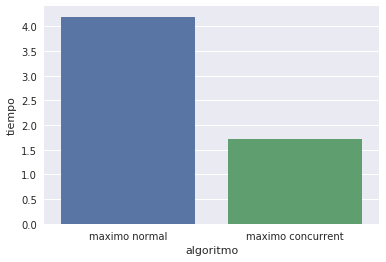
\includegraphics[width=0.8\textwidth]{imagenes/maxvsmax.png}
\end{center}

En este grafico se puede ver la comparación entre las dos implementaciones de maximo funcionando
para 5 archivos con 5 threads. Se puede ver claramente que la implementación concurrente
es más del doble de rapida.

\begin{center}
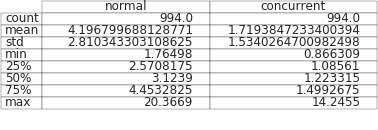
\includegraphics[width=0.8\textwidth]{imagenes/descplot.png}
\end{center}

En esta tabla se pueden ver los valores estádisticos de la comparación. Se
corrieron mil veces los algoritmos para este caso.

\begin{center}
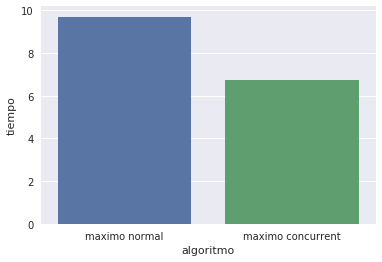
\includegraphics[width=0.8\textwidth]{imagenes/maxvsmax1thread.png}
\end{center}

Aquí se puede ver la comparación de ambos para 11 archivos con 1 solo thread.\\
Este resultado a priori es extraño ya que ambas se ejecutan de forma no concurrente. Sin embargo, al tener en cuenta que la versión no concurrente crea un hashmap para luego pasarlo a otro hashmap y ahí calcular el máximo, tiene sentido pensar que pueda haber demorado mayor cantidad de tiempo que su equivalente concurrente.

\begin{center}
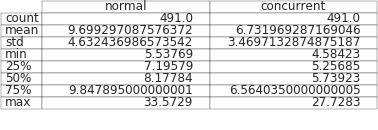
\includegraphics[width=0.8\textwidth]{imagenes/descplot2.png}
\end{center}

En esta tabla se pueden ver los valores estadísticos de la comparación, en este caso
los algorimos se corrieron 500 veces.

\subsection{Experimentación Threads}

Además, se realizó una experimentación corriendo ambas instancias variando la cantidad de threads con 1 $\leq n \geq 10$.
Ambas implementaciones se corrieron 500 veces para cada $n$ y se promediaron los tiempos arrojando los siguientes resultados:

\begin{center}
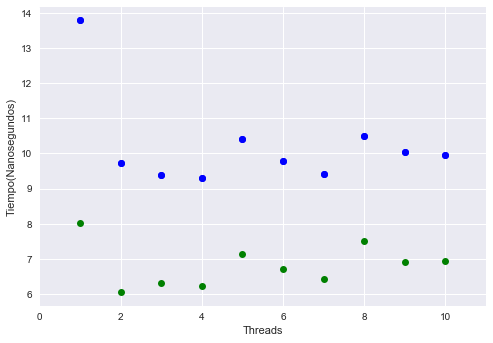
\includegraphics[width=0.8\textwidth]{imagenes/threads.png}
\end{center}

Donde el verde representa a la versión concurrente y el azul a la no concurrente.

Como esperabamos, encontramos que la versión concurrente arroja tiempos menores que su contraparte no concurrente. Sin embargo, se puede observar que al aumentar los threads no mejora los tiempos significativamente, de hecho en algunos casos los empeora. Esto podría tratarse a que al agregar palabras en la estructura se bloquean con un mutex las listas, haciendo mayores los tiempos de espera al haber muchos threads.

Por otro lado, a simple vista parece haber una correlación entre los tiempos.



\newpage
\section{Conclusión}
En este trabajo práctico se implementó la estructura ConcurrentHashMap de forma concurrente y no concurrente.
Además de obtener una noción práctica de conceptos y estructuras de datos para concurrencia vistas en la materia como Atómicos y Mutex, se pudo observar experimentalmente como afecta la performance de un programa al ser ejecutado de forma concurrente.

Tal como suponíamos, las distintas funciones en su versión concurrente se desempeñaron mejor que sus equivalentes no concurrentes comprobando
asi que nuestra hipótesis inicial era correcta.



\end{document}
